\documentclass[10pt]{beamer}

\usetheme{m}

\usepackage{booktabs}
\usepackage[scale=2]{ccicons}

%\usepackage{pgfplots}
%\usepgfplotslibrary{dateplot}

\usepackage[latin1]{inputenc}
\usepackage[spanish]{babel}

\usepackage{listings}
\usepackage{pgfplots}

\usepackage{amsmath}

\title{Ejemplo de aplicaci�n MPI}
\subtitle{C�lculo del valor aproximado de $2\pi$}
\date{}
\author{Luis Mar�a Costero Valero\\Jes�s Javier Dom�nech Arellano\\Hristo
  Ivanov Ivanov}
\institute{18 Enero 2016}

\titlegraphic{\hfill
\includegraphics[scale=0.2]{mpi.jpg}}

\definecolor{bgg}{HTML}{FBFBFB}
\def\gcolor{bgg}    % while presenting
%\def\gcolor{black} % while developing

\def\tikzpicdim{
  \draw[step=0.1cm, color=\gcolor] (0,-1) grid (12,7);
  \draw[step=1cm, color=\gcolor] (0,-1) grid (12,7);
}

\let\tikzpicdimlarge\tikzpicdim

\def\myurl{\hfil\penalty 100 \hfilneg \hbox}

\metroset{titleformat=regular}
\metroset{inner/sectiontitleformat=regular}
\metroset{outer/frametitleformat=regular}
\metroset{block=fill}

\lstset{%
  %backgroundcolor=\color{yellow!20},%
    basicstyle=\tiny\ttfamily,%
    numbers=left, numberstyle=\tiny, stepnumber=1, numbersep=5pt,%
    frame=l%
    }%


\begin{document}

\maketitle

%%======= INDICE ========================================
%\begin{frame}
%  \frametitle{�ndice}
%  \setbeamertemplate{section in toc}[sections numbered]
%  \tableofcontents[hideallsubsections]
%\end{frame}

%\section{Introduction} %=== Esrto genera una p�gina de secci�n.

\begin{frame}
  \frametitle{Problema}
  \emph{
    El problema computacional que hemos propuesto para este trabajo es
    calcular el valor aproximado de $\pi$.
  }
  \small
  \begin{align*}
    \int_{-\infty}^{\infty}\int_{-\infty}^{\infty}e^{-(x^2+y^2)/2}\mathit{dxdy}\approx \\ 
    \int_{-x_N}^{x_N}\int_{-y_M}^{y_M}e^{-(x^2+y^2)/2}\mathit{dxdy}\approx \\
    \sum_{i=0}^{N}\sum_{j=0}^{M}h^2e^{-(x^2+y^2)/2} 
    \approx 2\pi 
  \end{align*}
  \begin{align*}
    x_i = -x_N + ih, \qquad i=0,...,N. \\
    y_j = -y_M + jh, \qquad j=0,...,M. 
  \end{align*}
  \normalsize

\end{frame}


\begin{frame}[fragile]
  \frametitle{Problema -- Funci�n}
    \begin{tikzpicture}
    \tikzpicdimlarge
    \begin{onlyenv}<1->
    \node at (0.5,6) {
      \begin{minipage}{0.9\textwidth}
  \begin{center}
    \begin{tikzpicture}
      \begin{axis}
        \addplot3[
        mesh,
        samples=50,
        domain=-3:3,
        ] 
        {e^(-(x^2 + y^2)/2)};
      \end{axis}
    \end{tikzpicture}
  \end{center}
        \end{minipage}
      };
    \end{onlyenv}
\begin{onlyenv}<2->
    \node at (0.5,1.9) {
\begin{minipage}{0.9\textwidth}
\begin{lstlisting}[language=C]
for(i=long_rang*mi_rango;i<long_rang*(mi_rango+1);i++){
    x=-(xp/2)+i*h;
    for(k=0;k<num_div;k++){
        y=-(yp/2)+k*h;
        z=-0.5*(x*x+y*y);
        z= exp (z);
        total=total+h*h*z;
}}
\end{lstlisting}
 \end{minipage}
};
 \end{onlyenv}

 \end{tikzpicture}

\end{frame}

\begin{frame}[fragile] 
  \frametitle{Problema -- C�digo MPI}
  \emph{
    Utilizando MPI dividimos el intervalo a integrar en trozitos que son
    repartidos entre las diferentes m�quinas.
  }
  \begin{lstlisting}[language=C,basicstyle=\tiny]
/*............................*/
MPI_Init(&argc,&argv);
MPI_Comm_rank(MPI_COMM_WORLD,&mi_rango);
MPI_Comm_size(MPI_COMM_WORLD, &p);
if(mi_rango==0){
  // En caso de ser el nodo maestro, repartir el trabajo entre los nodos.
  for(w=1;w<p;w++)
    MPI_Send(&long_rang,1,MPI_LONG_DOUBLE,w,tag,MPI_COMM_WORLD);
    MPI_Send(&h,1,MPI_LONG_DOUBLE,w,tag,MPI_COMM_WORLD);
}else{
  // En caso contrario recibir la carga de trabajo asignada.
  MPI_Recv(&long_rang,1,MPI_LONG_DOUBLE,0,tag,MPI_COMM_WORLD,&status);
  MPI_Recv(&h,1,MPI_LONG_DOUBLE,0,tag,MPI_COMM_WORLD,&status);}

total = calculaPI();

/* Calcular el intervalo asignado. */

if(mi_rango==0){
  //Recibir la respuesta del resto de nodos.
  for(w=1;w<p;w++){
    MPI_Recv(buf,1,MPI_LONG_DOUBLE,w,tag,MPI_COMM_WORLD,&status);
    total=total+buf[0];}
}else{
  //Enviar la infomacion al nodo maestro.
  MPI_Send(&total,1,MPI_LONG_DOUBLE,0,tag,MPI_COMM_WORLD);}

MPI_Finalize();
  \end{lstlisting}
\end{frame}

\begin{frame}[fragile] 
  \frametitle{Resultados}
  \emph{
    Finalmente podemos observar los resultados obtenidos.
    \vspace*{30px}
    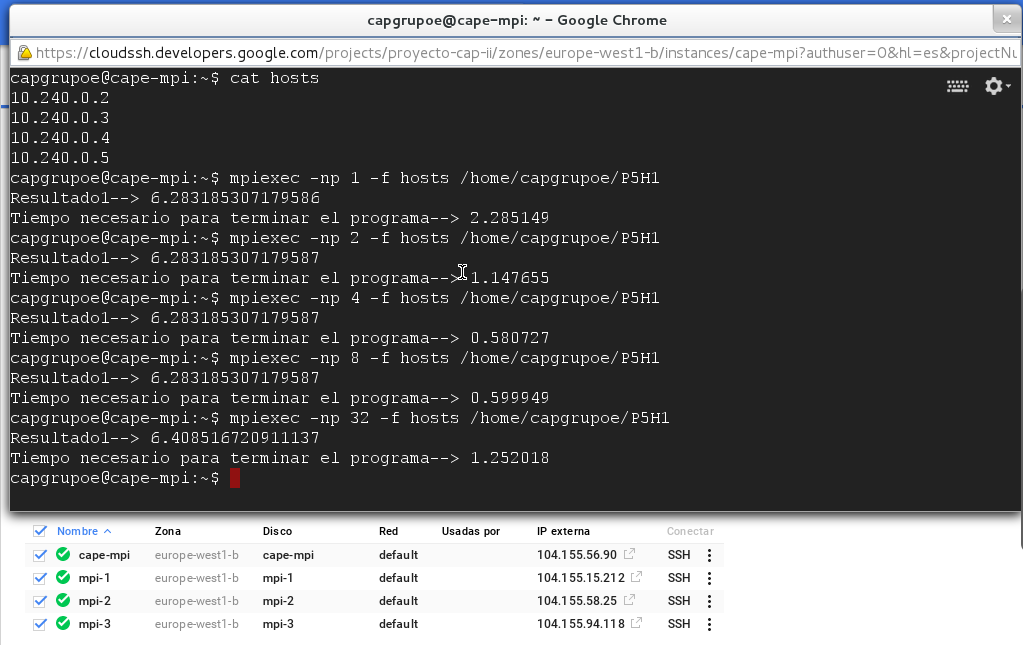
\includegraphics[scale=0.3]{resultado.png}
  }
\end{frame}

\end{document}
